% EBMAS (boztepe sachen // http://www.ebmas.net/deutsch/kampfstile/kampfstile_wingtzun.html):
%Die vier Wege der "Kraft":
%Im Umgang mit der "Kraft" gibt es vier Prinzipien im Wing Tzun:
%1. Befreie dich von deiner eigenen "Kraft"
%2. Befreie dich von der "Kraft" deines Gegners
%3. Nutze die "Kraft" des Gegners
%4. Fuege deine eigene "Kraft" zur "Kraft" des Gegners hinzu.

%Die 3 Teile des Wing Tzun Trainings
%1. Formen
%2. Chi Sao (Klebende Arme)
%3. Lat Sao (Sparring-Uebungen)

%5 distanzen
%1. Phase - Kaempfen mit den Fuessen (Trittdistanz)
%2. Phase - Kaempfen mit den Haenden (Schlagdistanz)
%3. Phase - Kaempfen mit Knie und Ellbogen
%4. Phase - Halten, Werfen, Gegenwerfen, Wuergen
%5. Phase - Bodenkampf 

% anstatt kontaktreflex => tastreflex

%Aufbau des Unterricht: Alphabet, Wort, Satz, Freier Dialog
%   (Basis, Form, Lat-sao, Freikampf)

% TODO kettenfauststoesse!
% TODO zentrallinie, dreieck

\documentclass[a4paper,12pt]{scrartcl}
\usepackage[austrian]{babel}
\usepackage[latin1]{inputenc}
\usepackage{hyperref}

\usepackage{graphicx}
\usepackage{url}
\DeclareGraphicsRule{.tif}{png}{.png}{`convert #1 `dirname #1`/`basename #1 .tif`.png}

\usepackage[font=small,format=plain,labelfont=bf,up,textfont=it,up]{caption}

\title{WingTsun Einsteiger Kompendium}
\author{Christoph Pickl\footnote{christoph.pickl@gmail.com}}

\newenvironment{techniken}
	{\begin{enumerate}}
	{\end{enumerate}}
\def\technik#1#2#3 {\item \textbf{#1} (\textit{#2}) #3}


% TODO kung fu definition:
% Kung fu or gongfu or gung fu.(??, Pinyin: g?ngfu) is a Chinese term often used in the West to refer to Chinese martial arts.[1] Its original meaning is somewhat different, referring to one's expertise in any skill achieved through hard work and practice, not necessarily martial. The Chinese literal equivalent of "Chinese martial art" would be ???? zh?nggu� w?sh�.[2]
% the strengthening of the body and the mind, the learning and the perfection of one's skills - rather than to what was being trained. Someone with "bad kung fu" simply has not put enough time and effort into training, or seems to lack the motivation to do so. Before the 1960s, Chinese martial arts was primarily referred to in the West as "Chinese boxing", rather than "kung fu". (hong kong films, bruce lee erstmals wort kung fu bekannt gemacht)

\begin{document}

\maketitle
%%%%%%%%%%%%%%%%%%%%%%%%%%%%%%%%%%%%%%%%%%

\subsection*{Vorwort}
%%%%%%%%%%%%%%%%%%%%%%%%%%%%%%%%%%%%%%%%%%

Dieses kleine Kompendium wurde w\"ahrend der anf\"anglichen Zeit an meiner Schule der EWTO\footnote{http://www.ewto.at} im sechsten Wiener Bezirk niedergeschrieben. Es dient vor allem Neueinsteiger als erste Orientierungshilfe und gibt \"Uberblick \"uber diese Kampfkunst. Es beinhaltet den obligatorischen historischen Hintergrund und allgemeine Informationen \"uber WingTsun, sowie eine Beschreibung der verschiedenen Techniken die angewendet werden.

Da dies sich jedoch lediglich mehr als eine Art \textit{Notiz} versteht als ein Fachbuch, kann leider keine Gew\"ahrleistung auf Korrektheit gegeben werden. Bei Anmerkungen jeglicher Art ist eine kurze Mail immer willkommen.

\tableofcontents
%%%%%%%%%%%%%%%%%%%%%%%%%%%%%%%%%%%%%%%%%%

\newpage

\section{Hintergrundinformationen}
%%%%%%%%%%%%%%%%%%%%%%%%%%%%%%%%%%%%%%%%%%
%%%%%%%%%%%%%%%%%%%%%%%%%%%%%%%%%%%%%%%%%%

Wing Chun ( \textit{Ving Tsun}, \textit{Wing Tsun}, \textit{Wing Tzun} oder auch \textit{Wyng Tjun} geschrieben\footnote{bez\"uglich der verschiedenen Schreibweisen und deren Bedeutung siehe Kapitel \ref{sec:verschstile}}) ist eine s\"udchinesische Kampfkunst und Selbstverteidigungsart  f\"ur den realen (Nahkampf-) Einsatz. Die Worte k\"onnen \"ubersetzt in so etwas wie ``sch\"oner Fr\"uhling''.
% aus dem 19.~Jahrhundert
%(siehe Kapitel~\ref{sec:prinzipien} auf Seite~\pageref{sec:prinzipien}) 

\subsection{Entstehungsgeschichte}
%%%%%%%%%%%%%%%%%%%%%%%%%%%%%%%%%%%%%%%%%%

Eine Legende besagt, dass --zusammengefasst gesagt-- eine Nonne diese Kampfkunst entwickelte und setzt somit keine \"uberlegene K\"orperkraft voraus, denn es verwendet die Kraft des Gegners f\"ur seine eigene Zwecke.
% TODO laut boztepe: Die Kampfkunst Wing Tzun wurde vor mehr als 250 Jahren in China von der Nonne Ng Mui und der sch\"onen Yim Wing Tzun entwickelt, die dieser Kampfkunst ihren Namen gab.

Eine l\"angere Variante dieser Erz\"ahlung besagt, dass in Zeiten des Krieges mehr K\"ampfer ben\"otigt wurden. Eines Tages versammelten sich eine Gruppe von Meistern um eine Kampfkunst zu entwickeln welche hoch effektiv war, aber auch schnell zu erlernen war; man bedenke dass eine traditionelle Shaolin Kung Fu/Wu Shu Ausbildung 18~intensive Jahre dauert! Alle Meister wurden jedoch umgebracht, und nur eine Frau (vermutlich eine Nonne) konnte das Wissen retten, in dem sie es einem kleinen M\"adchen weitergab. Dieses M\"adchen hatte den Namen \textit{Wing Chun}.

Einer der bekannteren Vertreter von Wing Chun ist \textit{Ip Man} (manchmal auch \textit{Yip Man} geschrieben) und ist zugleich der hoch angesehene Gro{\ss}meister in der EWTO; er selbst hatte immer auf Titeln wie ``Meister'' oder ``Gro{\ss}meister'' verzichtet. Hier sei auf den gleichnamigen Film hingewiesen, der f\"ur jeden waschechten Wing Chun'ler ein Muss ist.

\begin{figure}[htbp]
	\centering
	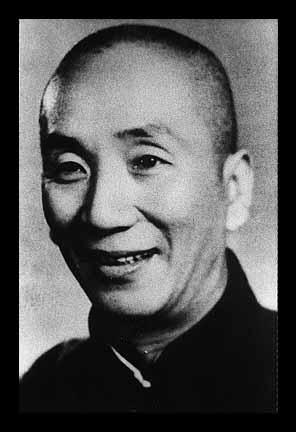
\includegraphics[width=5cm]{image/ip_man}
	\caption{Portraitfoto von Ip Man (Nov.~1893 -- Dez.~1972)}
	\label{img:ip_man}
\end{figure}

% http://www.ebmas.net/deutsch/kampfstile/kampfstile_wingtzun_yipman.html

\subsection{Verschiedene Stile}\label{sec:verschstile}
%%%%%%%%%%%%%%%%%%%%%%%%%%%%%%%%%%%%%%%%%%

Nachdem Ip Man verstorben war entwickelten sich viele verschiedene Stile von Wing Chun, und es entstanden aus Probleme der \"Ubersetzung als auch aus politischen Gr\"unden verschiedene Namen. Im Laufe der immer intensiveren Kommerzialisierung wurden manche Schreibweisen als Warenzeichen angemeldet, und somit gibt es eine Vielzahl von Schreibweisen.

Man kann sagen dass es drei Hauptschreibweisen gibt:

\begin{itemize}
	\item \textbf{Ving Tsun} -- Dies ist die internationale Schreibweise die auch Ip Man selbst verwendete. Eine der gr\"o{\ss}ten Vertreter ist ``The Ving Tsun Athletic Organization''.
	\item \textbf{Wing Chun} -- In Europa hat sich diese Form durchgesetzt, und wurde auch von Ip Mans Nachfahren verwendet.
	\item \textbf{WingTsun} -- Gesch\"utzt durch Leung Ting von der ``\textbf{I}nternational \textbf{W}ing \textbf{T}sun \textbf{A}ssociation'', mit lokalem Vertreter Keith R. Kernspecht von der ``\textbf{E}uropean \textbf{W}ing\textbf{T}sun \textbf{O}rganisation''. Leung Ting war der letzte Student von Ip Man bevor dieser verstarb.
%	\item \textbf{Traditional Wing Chung} -- Gesch\"utzt durch William Cheung von der ``World Wing Chun Kung Fu Association''. Er lernte damals 1950 eine sehr un\"ahnliche Art Wing Chung von Ip Man.
\end{itemize}
% oder auch: Wing Tzun
% quelle: http://www.dragonslist.com/threads/wing-chun-wing-tsun-ving-tsun-what-is-happening.1908/

%		=> kompendium verwendet weiters nur mehr WT/WingTsun, auch um den unterschied zu anderen stilen herzustellen (da evtl so manches speziell fuer das WingTsn, also Leung Ting/IWTA/ETWO ist), und evtl passts nicht zu anderen stilen
% TODO TODO TODO

Andererseits sollte man diesen Details nicht all zu viel Bedeutung geben, aus Gr\"unden die folgender Internetuser schon sehr gut erk\"arend dargelegt hat:

``\textit{That says Wing Chun in cantonese \ldots you can also see it romanized as Ving Tsun. Wing Tsun. And on and on. The spelling thing is more of a personal preference/political thing. Don't put a whole lot of emphasis on that.
The important thing to look for in a WC/VT/WT school is are they doing good martial art? It shouid be simple (not flashy) direct, practical, have economy of motion, use no brute force (use opponent's force against him)}''\footnote{\url{http://www.martialtalk.com/forum/showpost.php?p=1384420&postcount=2}}

\subsection{Graduierungssystem}
%%%%%%%%%%%%%%%%%%%%%%%%%%%%%%%%%%%%%%%%%%

12 Sch\"ulergrade, 12 Meistergrade (4 Techinker, 6 Praktiker).
Uniform: Grau, Abzeichen. Rot, dann Gelb (Philosoph).
Pr\"ufungen werden w\"ahrend (kostenpflichtige) Lehrg\"ange oder anderen speziellen Trainings (Intensivwoche) abgehalten. Sie kosten zwischen 15 und 25 Euro (je nach Grad) und laufen eigentlich fast so ab wie ein normales Training ohne speziellen ``Zur-Schau-Stellungen''.


\begin{figure}[htbp]
	\centering
	\begin{tabular}{cccc}
		\textsf{Sch\"uler} & \textsf{Ausbilder} & \textsf{Techniker} & \textsf{Meister} % TODO grossmeister /gelb
		\\
		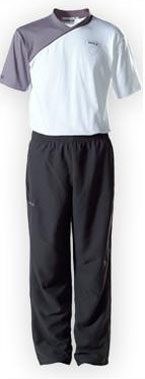
\includegraphics[width=3cm]{image/uniformen/schueler} &
			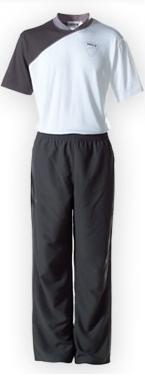
\includegraphics[width=3cm]{image/uniformen/ausbilder} &
			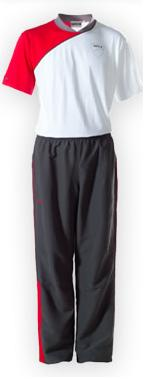
\includegraphics[width=3cm]{image/uniformen/techniker} &
			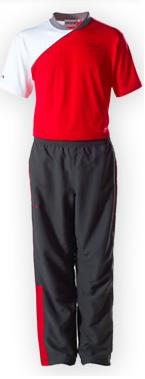
\includegraphics[width=3cm]{image/uniformen/meister}
	\end{tabular}
	\caption{Uniformen f\"ur die verschiedene Graduierungen der EWTO}
\end{figure}

%http://www.wingtsun.de/graduierung/wingtsun-schuelergrad.html
%http://wing-tsun.org/informationen/wing-tsun/pruefungen-und-graduierungen/


%1st - 4th, Learning fundamentals across the three ranges.
%5th - 8th, Ranges applied with movement and transition.
%9th - 12th, Application of the style, against kicks.

\begin{enumerate}
	\item Sch\"ulergrad \newline% Grad 1
	Grundlegende Haltung und Bewegung, Lap/Punch (BlitzDefence~1), Pak/Punch (BlitDefence~2) die \textit{Bong Gerk} Fusstechnik und der erste Teil der \textit{Siu Nim Tau} Form (Satz 1 bis 3).
% TODO blitz defence 1 (links vorne, lap/punch) ? und 2 (rechts vorne, pak/punch)?
	\item Sch\"ulergrad \newline% Grad 2
	Alle 8~S\"atze der \textit{Siu Nim Tau} Form,  % TODO Long range fighting, with bridging
	\item Sch\"ulergrad \newline % Grad 3
	%TODO Transitioning from Long to mid-range attacks.
	\item Sch\"ulergrad \newline % Grad 4
	Anfang der \textit{Chum Kiu} Form.% TODO Transitioning from mid to short-range attacks
	\item Sch\"ulergrad \newline % Grad 5
	% TODO gleichzeitigkeiten (zwei haende gleichzeitig einsetzen, drei punkt kontrolle)?
	\item Sch\"ulergrad \newline % Grad 6
	% TODO Poon Sao? oder doch 8?
	\item Sch\"ulergrad \newline % Grad 7
	Chi Sao 1st attack.
	\item Sch\"ulergrad \newline % Grad 8
	Chi Sao.
	\item Sch\"ulergrad \newline % Grad 9
	%TODO Against a single attacker.
	\item Sch\"ulergrad \newline % Grad 10
	Kampf gegen mehrere Gegner.
	\item Sch\"ulergrad \newline % Grad 11
	Kampf gegen einen bewaffnenten Gegner.
	\item Sch\"ulergrad \newline % Grad 12
	Kampf gegen mehrere bewaffnete Gegner.
	
\end{enumerate}
% TODO TODO TODO TODO TODO TODO
%Instructor Grades:
%	1-4 techniker
%	4-8 praktiker
%	9-12 philosoph
	
% TODO bilder von abzeichen; gibt auch leadership zeugs

\subsection{Verglichen mit anderen Kampfstilen}
%%%%%%%%%%%%%%%%%%%%%%%%%%%%%%%%%%%%%%%%%%

WingTsun ist eine \textbf{Kung Fu} Art (manchmal auch ``Gong Fu'' oder auch ``Wu Shu'') und daher mit \textbf{Taiji} verwandt (auch Taiji Chuan oder Tai Chi genannt) da beide eine Art \textbf{Qigong} sind. Kung Fu ist eine nach au{\ss}en gerichtet/externe (da es eher harte Bewegungen gibt) und Taiji eine nach innen (weiche Bewegungen) gerichtete Qigong Art. WingTsun wird nachgesagt etwas ``mehr in der Mitte'' zu sein, da man die Energie des Angreifers nutzt und sich weich bewegt. Im Gegensatz zum \textbf{Shaolin Kung Fu} gibt es keine starr festgelegten Bewegungen, sondern man beruht mehr auf ein paar wenige, grundlegende (Kampf-)Prinzipien. Siehe Kapitel~\ref{sec:prinzipien}.

Eine weitere Gemeinsamkeit die sich WingTsun und Taiji teilen, ist die der Vorstellung dass unser K\"orper flie{\ss}en soll wie Wasser (unser K\"orper besteht ja auch immerhin aus rund 80\% Wasser). Er soll weich und nicht hart (keine harten Blocks die nur aufgrund von \"uberlegener Muskelkraft funktionieren wie bei \textbf{Karate}), locker und nicht verspannt sein (sonst bekommt man unter anderem nicht die notwendige Geschwindigkeit zusammen).
% TODO vs Kickboxer (Tritte)
% TODO  vs Boxen
% TODO  vs tae kwon do (korea)

\begin{figure}[htbp]
	\centering
	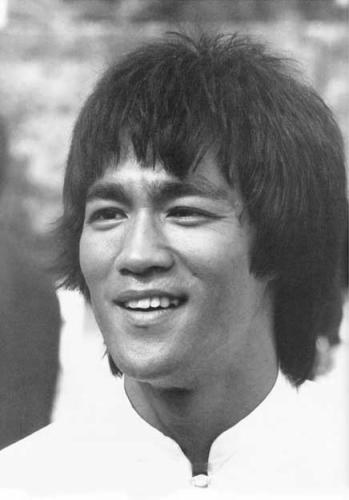
\includegraphics[width=5cm]{image/bruce_lee}
	\caption{Bruce Lee, popul\"arer Kung Fu K\"ampfer und Sch\"uler von Yip Man}
	\label{img:bruce_lee}
\end{figure}

%\subsection{Physiologie des Fauststo{\ss}}
%%%%%%%%%%%%%%%%%%%%%%%%%%%%%%%%%%%%%%%%%%
% TODO TODO TODO TODO TODO TODO

\newpage
\section{Techniken}
%%%%%%%%%%%%%%%%%%%%%%%%%%%%%%%%%%%%%%%%%%
%%%%%%%%%%%%%%%%%%%%%%%%%%%%%%%%%%%%%%%%%%

Grunds\"atzlich sollte man sich verinnerlichen dass vor allem (Kontakt-) Reflexe trainiert werden und man sich so bestimmte Bewegungen angew\"ohnt und automatisch ausf\"uhrt. Diese machen es einem sogar m\"oglich sich blind zu verteidigen, da nichts weiter n\"otig ist als der Kontakt zum Gegner; man bleibt quasi immer \textit{kleben}.

\subsection{Formen}
%%%%%%%%%%%%%%%%%%%%%%%%%%%%%%%%%%%%%%%%%%

In WT gibt es sechs Formen die es einem erm\"oglichen die Konzepte, Techniken und Theorien zu verstehen und selbst am eigenen K\"orper zu erleben. Vor allem den Konzepten sind eine gro{\ss}e Aufmerksamkeit zu schenken, da WT eigentlich auf diesen aufbaut, als auf einfach umzusetzende Techniken.

\paragraph{Freihand Formen:}
\begin{enumerate}
	\item \textbf{Siu Nim Tao} (auch ``Sil Lum Tao'' oder auch ``Siu-Lien-Tao'' genannt); bedeutet etwas wie ``Form der kleinen Idee'' im Sinne von Vorstellung.
%		=> http://www.sntform.com/tag/how-to-perform-siu-nim-tao/
%		=> http://en.wikipedia.org/wiki/Siu_Nim_Tao
	\item \textbf{Chum Kiu}; seeking/searching for the bridge
	\item \textbf{Biu Tze/Jee}; thrusting/darting fingers
	\item \textbf{Muk Yan Jong} Ist auch gleichzeitig der Name der Holzpuppe. Lernt man normalerweise erst mit einem h\"oheren Grad.

\begin{figure}[h]
	\centering
	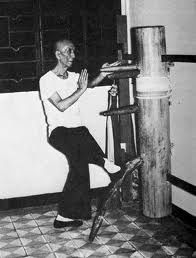
\includegraphics[width=5cm]{image/wooden_dummy}
	\caption{Yip Man in Verwendung einer Holzpuppe, einer Muk Yan Jong}
	\label{img:wooden_dummy}
\end{figure}

	% TODO TODO TODO TODO TODO TODO
\end{enumerate}

\paragraph{Formen mit Waffen:}
\begin{enumerate}
\setcounter{enumi}{4}
	\item \textbf{Luk Dim Boon Gwun} mit Langstab (in Englisch: Dragon Pole)
	\item \textbf{Bat Jam Dou} mit Doppelmesser
	% TODO TODO TODO TODO TODO TODO
\end{enumerate}


%subsection{Fussarbeit}
% TODO have a look at: http://www.brooklynwt.com/wing_tzun_footwork.htm

%\sub?subsection{Stand}
%%%%%%%%%%%%%%%%%%%%%%%%%%%%%%%%%%%%%%%%%%
%IRAS. front stand
% ausfuehrung:
%	kinn zurueck; lockerer, gerader oberkoerper; becken nach vorne
% 	fuesse:	1. fersen zusammen, spitzen nach aussen
%			2. auf den fussballen drehen, fersen auseinander
% 	knie tief mit spannung
% charakteristik: bildet ein dreieck, von oben linie durch kopf/huefte, eigene fuesse nicht mehr sichtbar
% sinn? zum beine trainieren & co, aber nicht wirklich zum einsatz im real

%\begin{figure}[htbp]
%	\centering
%	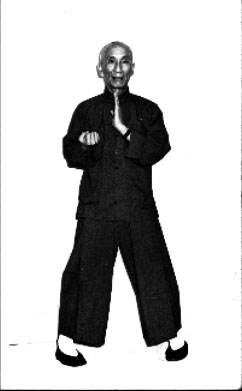
\includegraphics[width=5cm]{image/iras}
%	\caption{Der }
%	\label{img:ip_man}
%\end{figure}
% TODO TODO TODO TODO


\subsection{Prinzipien}\label{sec:prinzipien}
%%%%%%%%%%%%%%%%%%%%%%%%%%%%%%%%%%%%%%%%%%

Es gibt folgende \textbf{4 Leits\"atze} die das grunds\"atzliche Verhalten gut beschreiben\footnote{\url{http://www.wtrettigheim.de/news/prinzip.html}}:

%    If the way is free, hit or go through!
%    if the way is NOT free, stick with your hands (start to feel the opponent)
%    if the opponent is weaker , than follow 1, if stronger, be flexible and passive
%    if the opponent backs off, follow him closely until you succeed

% TODO vierte schliesst mit erstem wieder den kreis
%1. Wenn der Weg frei ist, stosse zu !
%2. Bekommst du Kontakt mit deinem Gegner, bleibe kleben !
%3. Ist die Kraft des Gegners groesser, gib (weich) nach !
%4. Wenn sich der Gegner zurueckzieht, folge ihm!

\begin{enumerate}
	\item \textit{Ist der Weg frei, stoss nach vorn!} \newline
		Man sollte immer zum Gegner zu Druck aus\"uben und auf ihn zugehen. Dies kostet nat\"urlich eines an \"Uberwindungskraft da man quasi dem Tod ins Auge schauen muss. Man darf nicht aus Angst oder Unentschlossenheit z\"ogern, als auch solte man nicht rein getrieben von Aggressivit\"at sein.
	\item \textit{Ist der Weg versperrt, bleib kleben!} \newline
		Das hei{\ss}t wenn der Angriff geblockt wurde, sollte man nicht wieder die Faust zur\"uckziehen, sondern am Hindernis haften bleiben. Dies ist ein wesentlicher Unterschied gegen\"uber vielen anderen Kampfstilen. Eine \"Ubung bei dem dieses Prinzip angewendet wird ist \textit{Chi Sao} (siehe Abbilung~\ref{img:chi_sao} auf Seite~\pageref{img:chi_sao}).
	\item \textit{Ist die Kraft des Gegners zu gro{\ss} (der Weg zu schwer), gib nach!} \newline
		Da Angreifer sich gerne kleinere und schw\"achere Gegner suchen, geht WT davon aus dieser wesentlich kraftvoller ist.\\ Deshalb gibt man bei weich und flexibel nach, um somit den Angriff ins Leere laufen zu lassen.
	\item \textit{Zieht sich der Gegner zur\"uck, folg ihm!} \newline
		Dies ist mit dem zweiten Prinzip verbunden, da sobald sich eine L\"ucke ergibt man wieder vorsto{\ss}en muss (WT ist als ein Nahkampfstil am besten in Faustdistanz anzuwenden).
\end{enumerate}

\begin{figure}[h]
	\centering
	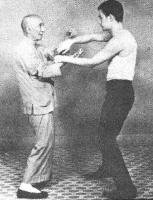
\includegraphics[width=5cm]{image/chi_sao.jpg}
	\caption{Yip Man beim Praktizieren des \textit{Chi Sao}, der klebenden H\"ande}
	\label{img:chi_sao}
\end{figure}

\subsection{Positionen}
%%%%%%%%%%%%%%%%%%%%%%%%%%%%%%%%%%%%%%%%%%

WT umfasst 18 grundlegende Techniken, davon gibt es folgende 6~Positionen:
% techniken / positionen
\begin{techniken}
	\technik{Bong Sao}{wing arm}{im Chi Sao}
	% Soeng/Siong Bong Sao (double wing arm)
	\technik{Fook Sao}{controlling/cover hand}{im Chi Sao}
	\technik{Man Sao}{seeking hand}{}
	\technik{Wu Sao}{sch\"utzende Hand}{wenn einarmige Ausf\"uhrung (Schlag), dann sollte zweite Hand diese Position einnehmen}
	\technik{Tan Sao}{absorbing/dispersing hand}{im Chi Sao}
	\technik{Kau Sao}{detaining hand}{}
\end{techniken}
% TODO siehe ordner: /_my_latex_kompendium -- www.wingchunonline.com
\subsection{Bewegungen}
%%%%%%%%%%%%%%%%%%%%%%%%%%%%%%%%%%%%%%%%%%
Weiters gibt es im WT ein Dutzend Namen f\"ur die Bewegungen:
% techniken / bewegungen
\begin{techniken}
	\technik{Jam Sao}{sinkende Hand}{bei Siu Nim Tao}
	\technik{Gaun Sao}{cultivating arm}{}
	\technik{Jut Sao}{choking hand}{}
	\technik{Huen Sao}{kreisende Hand}{}
	\technik{Lap Sao}{ziehende H\"ande}{BlitzDefence 1; im Kampfspiel}
	\technik{Pak Sao}{klatschende Hand}{BlitzDefence 2; im Kampfspiel}
	\technik{Tok Sao}{lifting hand}{}
	\technik{Lan Sao}{bar/barring arm}{}
	\technik{Tie Sao}{uplifting hand}{}
	\technik{Jip Sao}{receiving hand}{}
	\technik{Gum Sao}{dr\"uckende Hand}{}
	\technik{Biu Sao}{darting hand}{}
\end{techniken}
% Fat/Fut Sao (buddha hand)
% Gong Zau (downward elbow)
% Chi Sao (energy arms)

%\subsection{Kettenfauststo{\ss}}
%%%%%%%%%%%%%%%%%%%%%%%%%%%%%%%%%%%%%%%%%%
% TODO TODO TODO TODO TODO TODO

%\begin{appendix}
%\section{Appendix}
%%%%%%%%%%%%%%%%%%%%%%%%%%%%%%%%%%%%%%%%%%
%%%%%%%%%%%%%%%%%%%%%%%%%%%%%%%%%%%%%%%%%%

%\listoffigures

%\subsection{Schulordnung der EWTO}
%%%%%%%%%%%%%%%%%%%%%%%%%%%%%%%%%%%%%%%%%%

%\subsection{Referenzen}
%%%%%%%%%%%%%%%%%%%%%%%%%%%%%%%%%%%%%%%%%%
%weblinks
%	ewto.at
%	http://www.leungting.com
%	http://www.wtwatford.co.uk
%buecher

%\begin{thebibliography}
%\\
%\bibitem[Sha98]{Sha95} Adi Shamir (1995): \textsl{RSA for Paranoids}, 2.Auflage Addison-Wesley, New York
%\end{thebibliography}


%\subsection{Glossar}
%%%%%%%%%%%%%%%%%%%%%%%%%%%%%%%%%%%%%%%%%%
% Sao		Hand
% Kuen		Faust
% Gerk		Fuss/Bein
% Sifu		Meister
% Sigung		Des Meisters Meister
% Dan Tien/Tantien		Energiezentrum unter'm Bauchnabel
%\url{http://en.wikipedia.org/wiki/Wing_Chun_terms}
%\url{http://www.mainewingchunkungfu.com/Dictionary.htm}
%\end{appendix}

\end{document}